% !TeX encoding = UTF-8

\documentclass{protokol}

\usepackage{tikz}
\usetikzlibrary{calc}
\usetikzlibrary{arrows}

%====== Units =====
\usepackage{siunitx}
\sisetup{inter-unit-product =\ensuremath{\cdot}}
\sisetup{group-digits = integer}
\sisetup{output-decimal-marker = {,}}
\sisetup{exponent-product = \ensuremath{\cdot}}
\sisetup{separate-uncertainty}
\sisetup{tight-spacing = false}
%\sisetup{scientific-notation = true}
%\sisetup{round-mode=places,round-precision=4}
%\sisetup{evaluate-expression}


%====== Grafy =====
\usepackage{pgfplots}
\pgfplotsset{width=0.8\linewidth, compat=1.17}
\def\plotcscale{0.8}
\usepackage{pgfplotstable}
\usepackage[figurename=Graf]{caption} % figure caption rename
%====== Rovnice align block ======
\usepackage{amsmath}
\setlength{\jot}{10pt} % rozestup mezi řádky

\graphicspath{ {./img/} }

%====== Vyplňte údaje ======
\jmeno{Jakub Charvot}
\kod{240844}
\rocnik{2.}
\obor{MET}
\skupina{MET/4}
\spolupracoval{Radek Kučera}

\merenodne{10.\,11.\,2022}
\odevzdanodne{24.\,11.\,2022}
\nazev{Operační usměrňovače}
\cislo{4} %měřené úlohy

\predmet{Analogové elektronické obvody}
\ustav{Ústav mikroelektroniky}
\skola{FEKT VUT v Brně}

\def\para{x+0}
\def\parb{\para-80}

% CSV
\usepackage{blindtext}

\usepackage{subfiles} % Best loaded last in the preamble
\usepackage{datatool}

% \DTLloaddb[omitlines=2]{prvni}{data/prvni-cast.csv}
% \DTLloaddb[omitlines=2]{druha}{data/druha-cast.csv}



\begin{document}
	%====== Vygenerování tabulky ======
%	\maketitle
	%====== Úvodní texty protokolu ======

%	\section{Teoretický úvod}
%		\begin{figure}[h!]
    \centering
    
\includegraphics[width=\textwidth]{schema.png}
    \centering
    \caption{Schémata zapojení -- a) jednocestný usměrňovač, b) dvoucestný usměrňovač, c) dvoucestný usměrňovač s minimem přesných součástek.}
    \label{fig:schema}
\end{figure}



\subsection{Funkce jednotlivých zapojení}

    Operační zesilovač s OZ má za úkol překonat nedostatky, které má zapojení pouze s diodami, které díky svému prahovému napětí nedokáží usměrňovat velmi malá napětí. 
    
    Zapojení 1a) je jednocestný usměrňovač, kdy je vždy přes jednu diodu uzavřená záporná zpětná vazba a druhá dioda je uzavřená. Na výstupu je pak signál jednocestně usměrněný a invertovaný. 
    
    Zapojení 1b) pak tento signál zdvojnásobí a sečte s původním vstupním signálem, ve výsledku tedy původní záporné půlvlny zůstanou a kladné po sečtení odpovídají opět záporným. Výsledkem je tedy dvoucestně usměrněný invertovaný signál. 
    Nevýhodou tohoto zapojení je nutnost použít dva co nejshodnější odpory a k nim jeden, který odpovídá hodnotu přesně polovině, při nedodržení nebudou na výstupu půlvlny stejně velké, toto značně zdražuje zapojení. 

    Tento problém se snaží řešit zapojení 1c), kdy pro správnou funkci stačí jedna dvojice přesných odporů \( R_2\) a \(R_3\). Záporná zpětná vazba prvního OZ je vždy uzavřena přes druhý OZ, díky diodám je ale cesta zpětné vazby jiná pro kladný a pro záporný signál, takže ve výsledku je na výstupu druhého OZ signál vždy kladný, neboli dvoucestně usměrněný.   
%		
%	% \newpage
%	\section{Výsledky počítačové simulace}
%		\begin{figure}[h!]
    \centering
    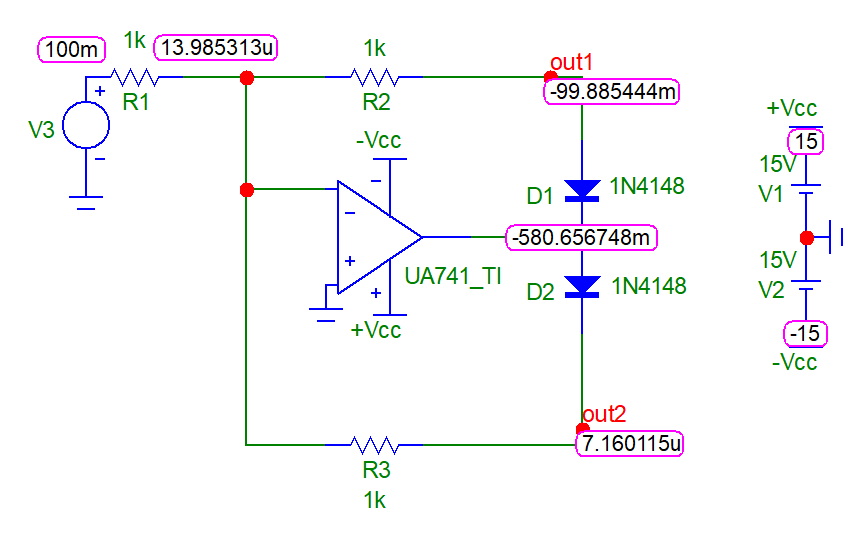
\includegraphics[width=0.63\textwidth]{microcap/1-dcbod.png}
    \caption{Zapojení a) -- stejnosměrný prac. bod pro kladné vstupní napětí.}
    \label{fig:microcap/.png}
\end{figure}

\begin{figure}[h!]
    \centering
    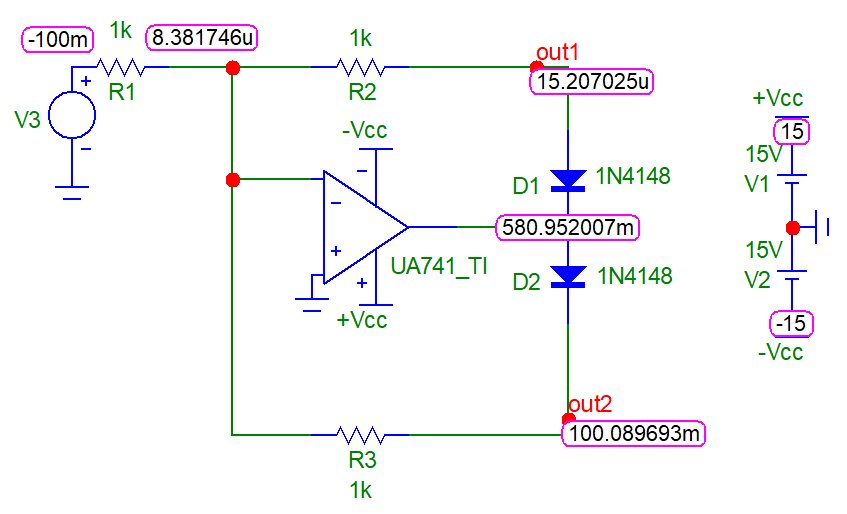
\includegraphics[width=0.63\textwidth]{microcap/1-dcbod2.png}
    \caption{Zapojení a) -- stejnosměrný prac. bod pro záporné vstupní napětí.}
    \label{fig:microcap/.png}
\end{figure}

\begin{figure}[h!]
    \centering
    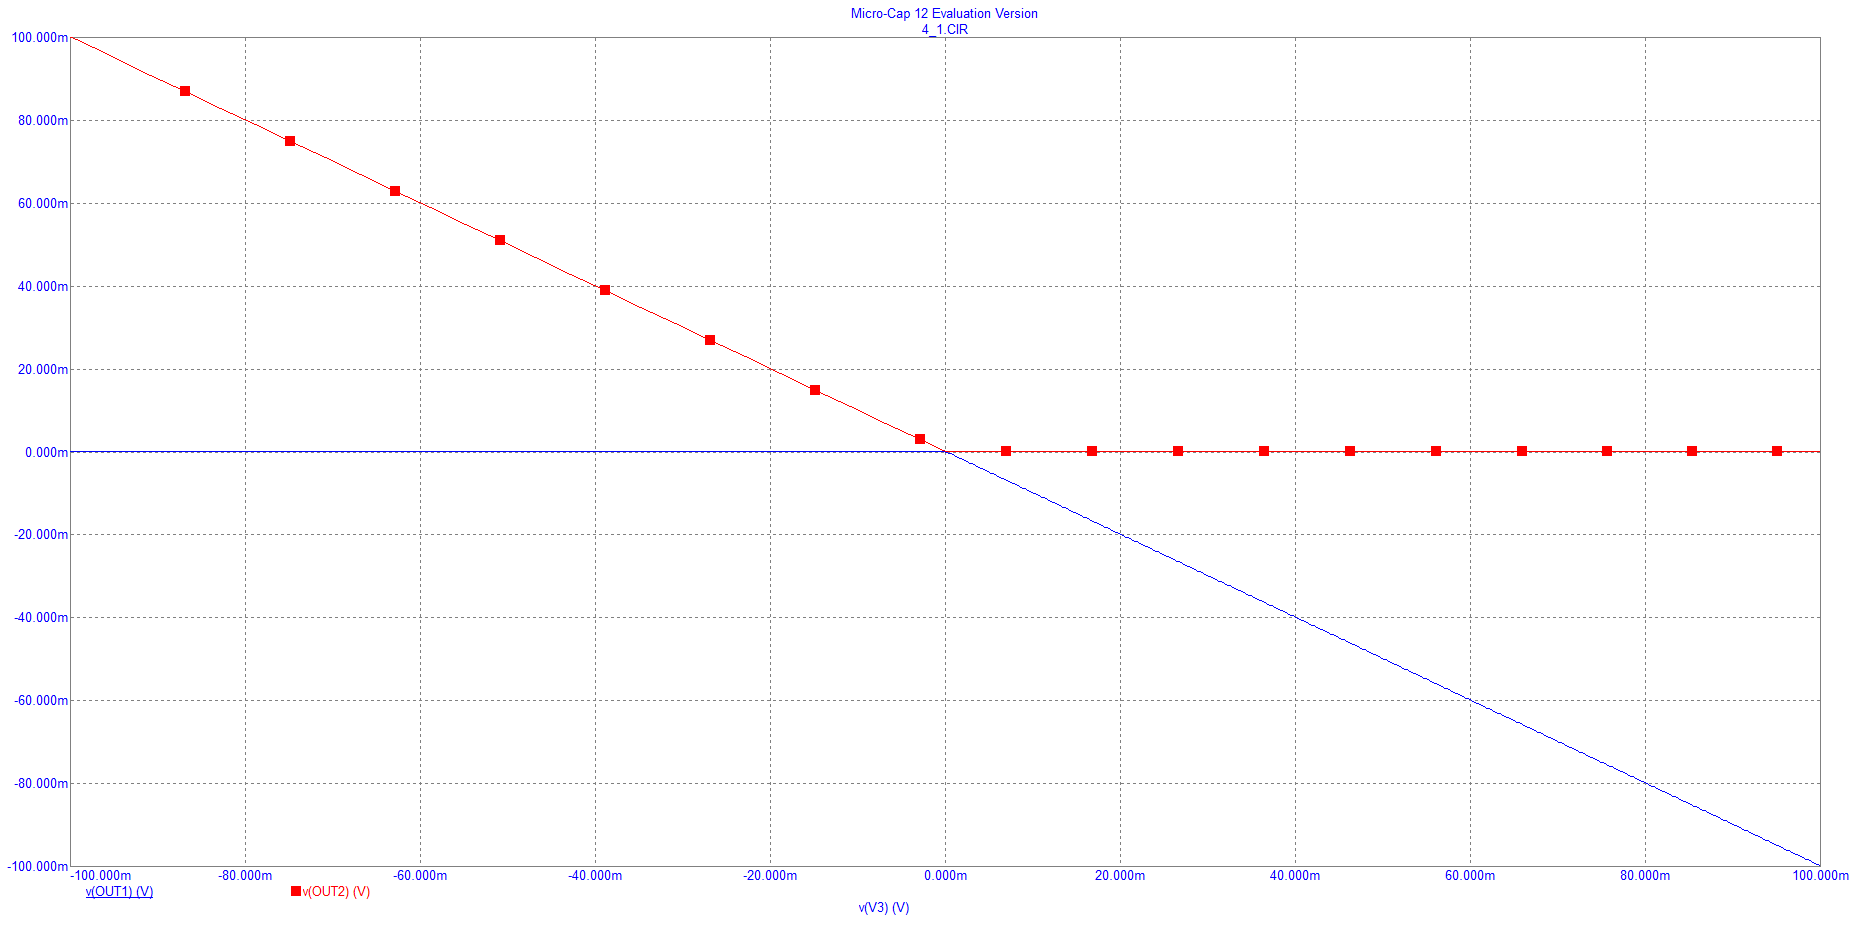
\includegraphics[width=0.8\textwidth]{microcap/1-dcprevodni.png}
    \caption{Zapojení a) -- stejnosměrná převodní charakteristika.}
    \label{fig:microcap/.png}
\end{figure}

\begin{figure}[h!]
    \centering
    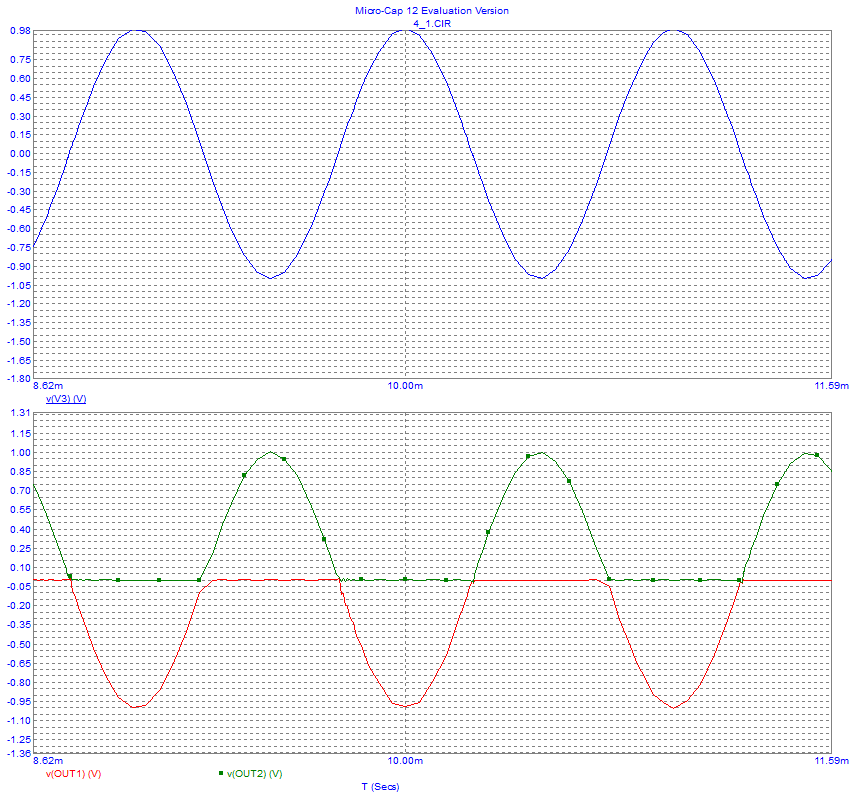
\includegraphics[width=0.8\textwidth]{microcap/1-transient-1khz-1v.png}
    \caption{Zapojení a) -- časová závislost obou výstupních napětí na vstupním napětí, jednocestné zesílení, \(f=\qty{1}{\kilo\hertz}, U_M=\qty{1}{\volt}\).}
    \label{fig:microcap/.png}
\end{figure}

\begin{figure}[h!]
    \centering
    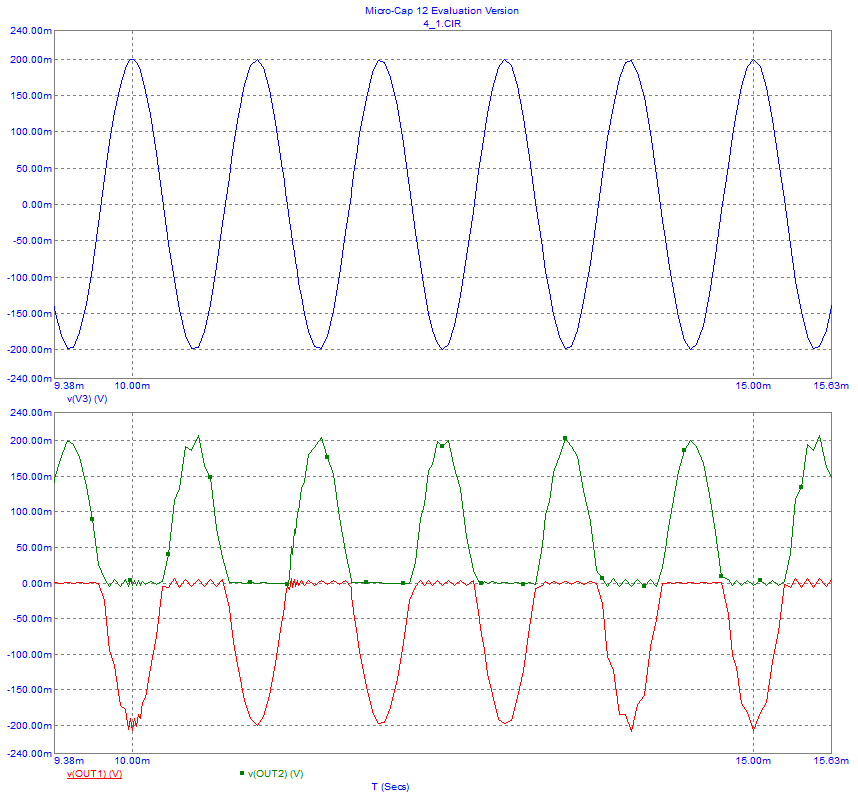
\includegraphics[width=0.7\textwidth]{microcap/1-transient-1khz-0.2v.png}
    \caption{Zapojení a) -- časová závislost obou výstupních napětí na vstupním napětí, nejmenší amplituda, při které zapojení obstojně usměrňuje, \(f=\qty{1}{\kilo\hertz}, U_M=\qty{200}{\milli\volt}\).}
    \label{fig:microcap/.png}
\end{figure}

\begin{figure}[h!]
    \centering
    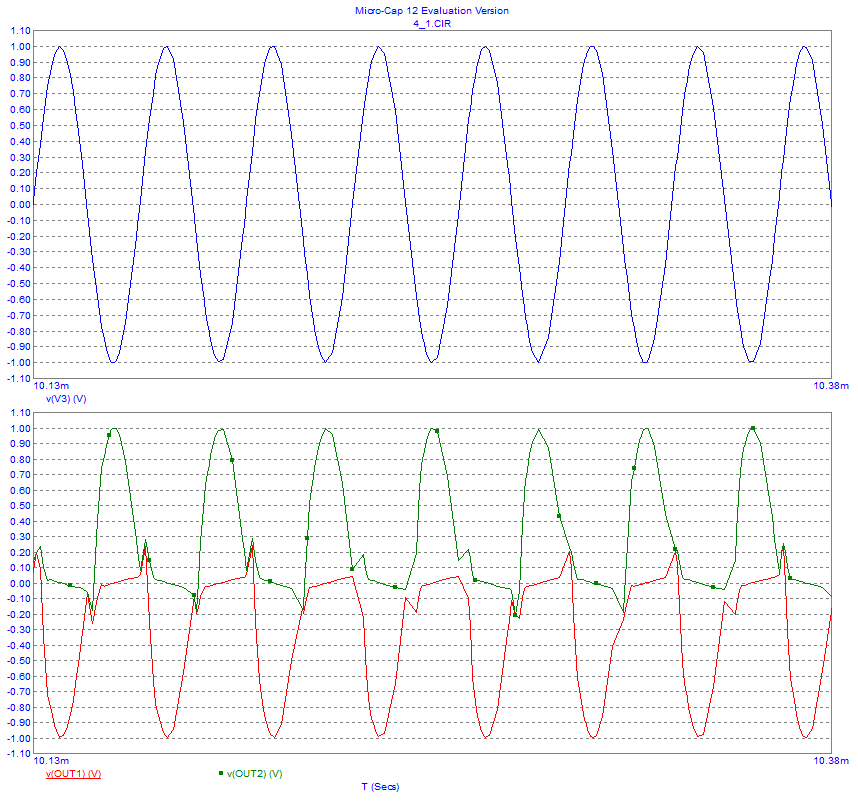
\includegraphics[width=0.7\textwidth]{microcap/1-transient-30khz-1v.png}
    \caption{Zapojení a) -- časová závislost obou výstupních napětí na vstupním napětí, nejvyšší frekvence, při které zapojení obstojně usměrňuje, \(f=\qty{30}{\kilo\hertz}, U_M=\qty{1}{\volt}\).}
    \label{fig:microcap/.png}
\end{figure}

\begin{figure}[h!]
    \centering
    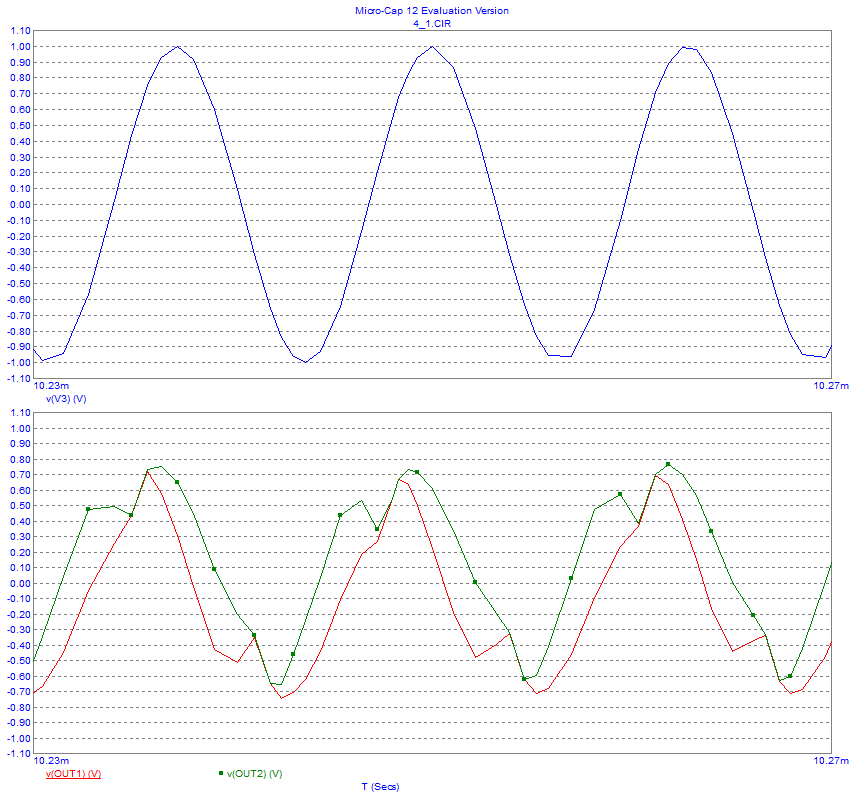
\includegraphics[width=0.8\textwidth]{microcap/1-transient-100khz-1v.png}
    \caption{Zapojení a) -- časová závislost obou výstupních napětí na vstupním napětí, příliš vysoká frekvence, k usměrnění nedochází vůbec, \(f=\qty{100}{\kilo\hertz}, U_M=\qty{1}{\volt}\).}
    \label{fig:microcap/.png}
\end{figure}    

% \begin{figure}[h!]
%     \centering
%     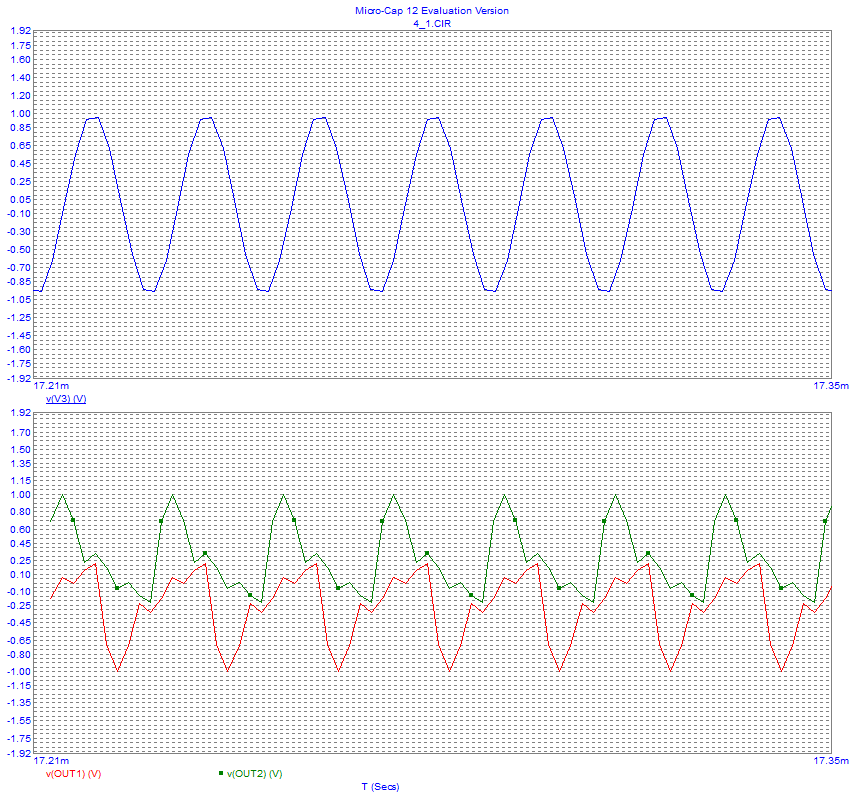
\includegraphics[width=0.8\textwidth]{microcap/1-transient-50khz-1v.png}
%     \caption{microcap/.png}
%     \label{fig:microcap/.png}
% \end{figure}

\begin{figure}[h!]
    \centering
    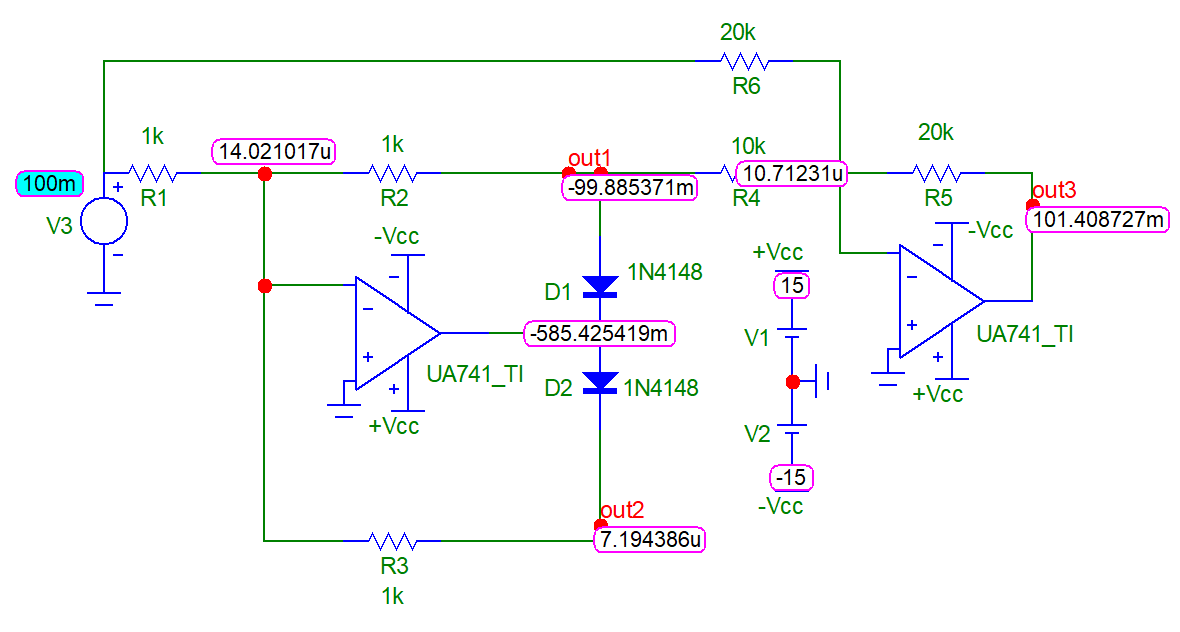
\includegraphics[width=0.8\textwidth]{microcap/2-dcbod.png}
    \caption{Zapojení b) -- stejnosměrný prac. bod při kladném napětí na vstupu, na výstupu kladné napětí.}
    \label{fig:microcap/.png}
\end{figure}

\begin{figure}[h!]
    \centering
    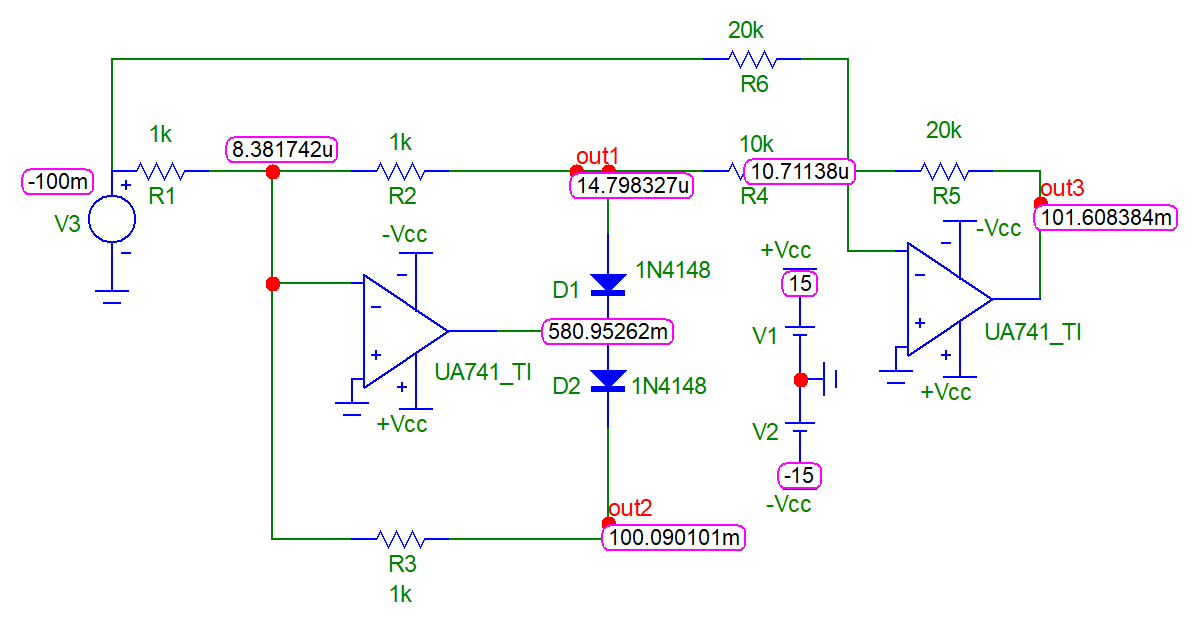
\includegraphics[width=0.61\textwidth]{microcap/2-dcbod2.png}
    \caption{Zapojení b) -- stejnosměrný prac. bod při záporném napětí na vstupu, na výstupu opět kladné napětí.}
    \label{fig:microcap/.png}
\end{figure}

\begin{figure}[h!]
    \centering
    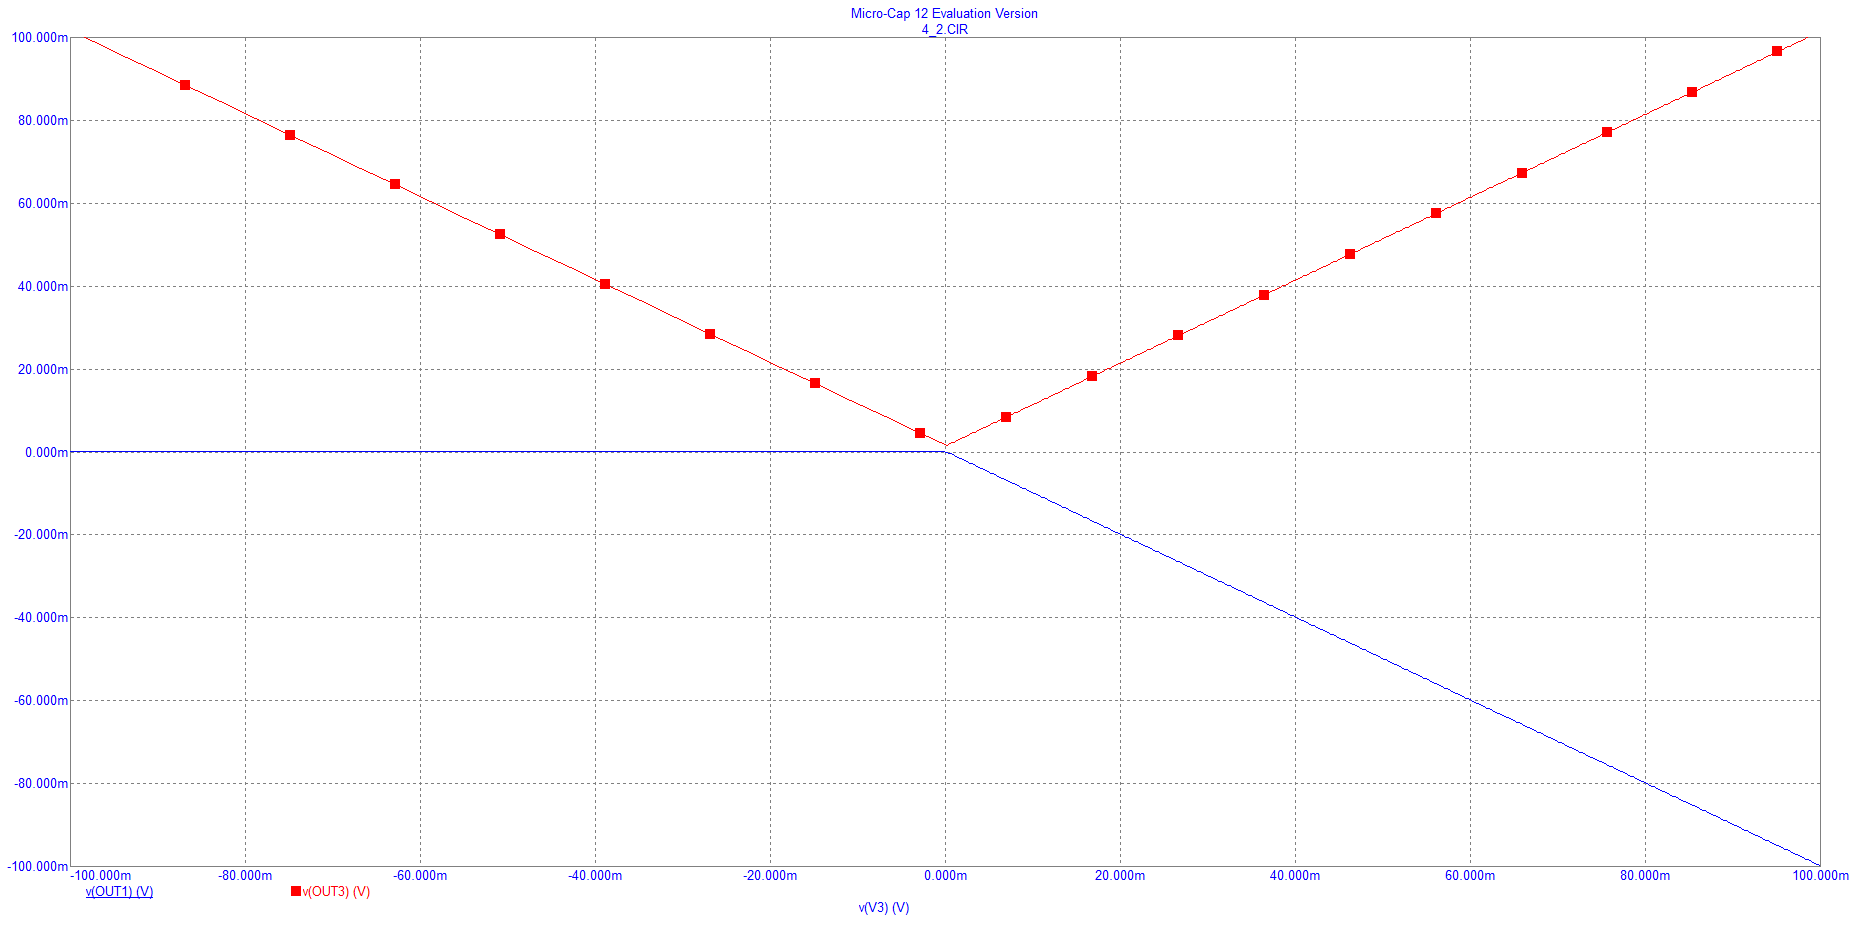
\includegraphics[width=0.61\textwidth]{microcap/2-dcprevodni.png}
    \caption{Zapojení b) -- stejnosměrná převodní charakteristika dvoucestného usměrnění.}
    \label{fig:microcap/.png}
\end{figure}

\begin{figure}[h!]
    \centering
    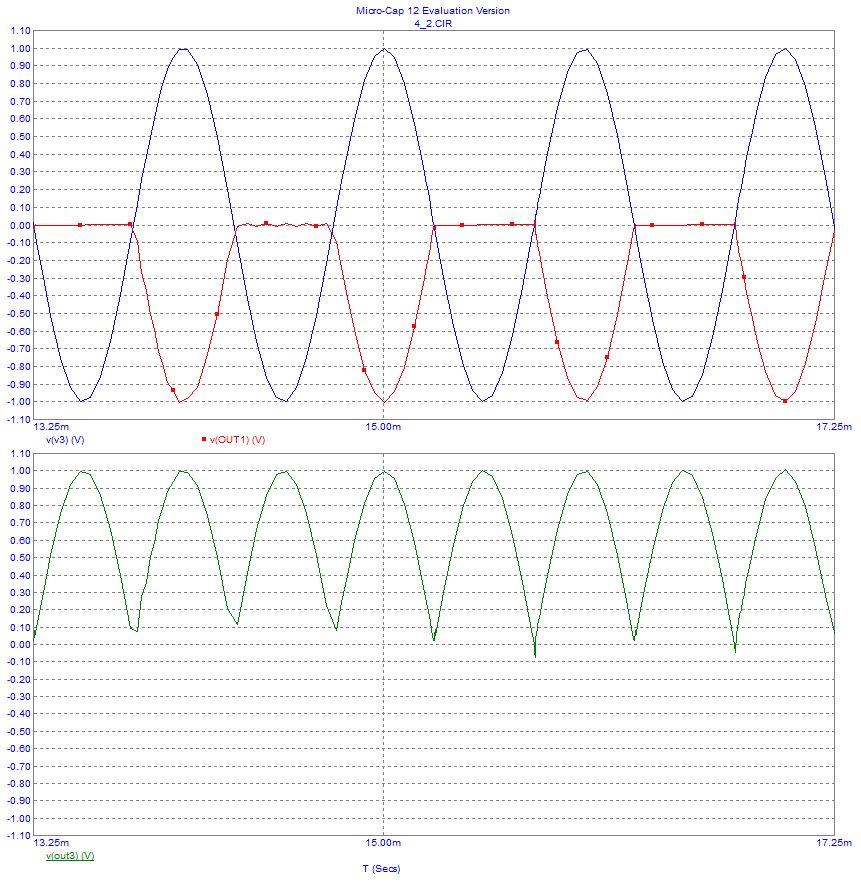
\includegraphics[width=0.61\textwidth]{microcap/2-transient-1khz-1v.png}
    \caption{Zapojení b) -- časová závislost napětí na výstupech obou OZ na vstupním napětí, jednocestné a dvoucestné usměrnění, \(f=\qty{1}{\kilo\hertz}, U_M=\qty{1}{\volt}\).}
    \label{fig:microcap/.png}
\end{figure}

% \begin{figure}[h!]
%     \centering
%     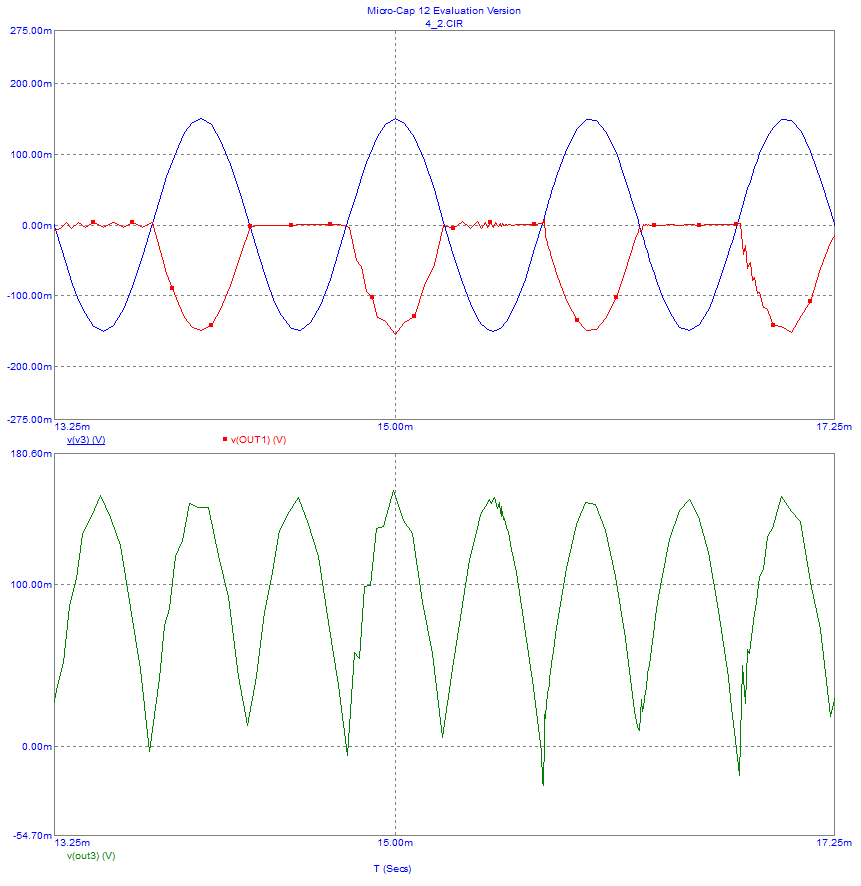
\includegraphics[width=0.8\textwidth]{microcap/2-transient-1khz-0.15v.png}
%     \caption{Zapojení b) -- časová závislost napětí na výstupech obou OZ na vstupním napětí, nejmenší amplituda, při které uspokojivě usměrňuje, \(f=\qty{1}{\kilo\hertz}, U_M=\qty{150}{\milli\volt}\).}
%     \label{fig:microcap/.png}
% \end{figure}

\begin{figure}[h!]
    \centering
    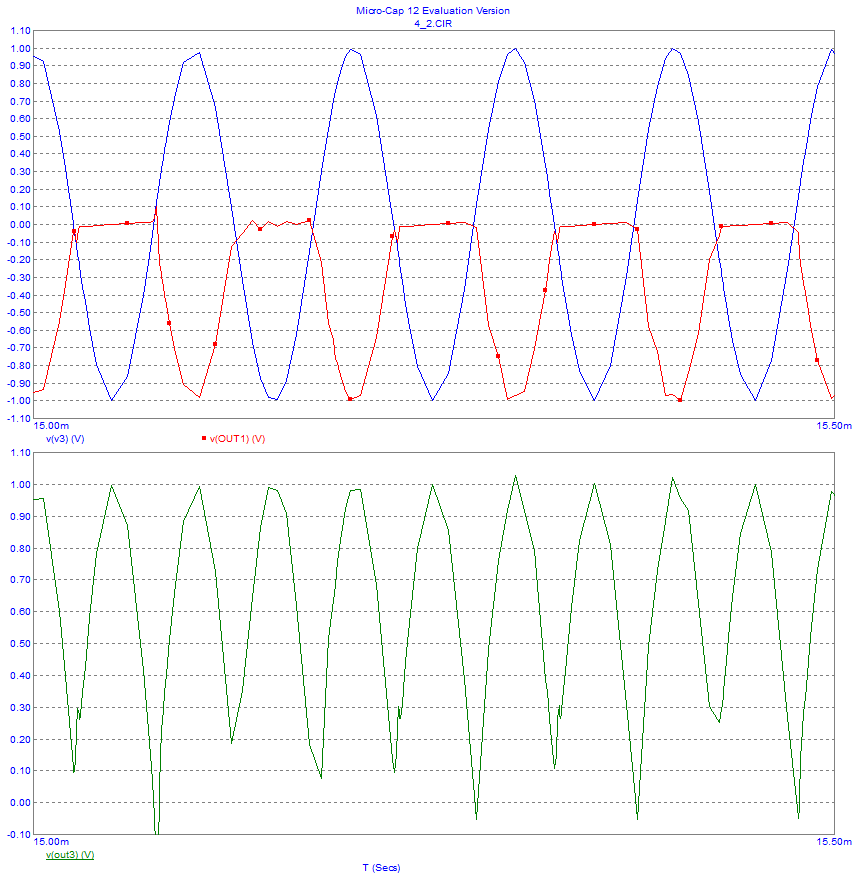
\includegraphics[width=0.7\textwidth]{microcap/2-transient-10khz-1v.png}
    \caption{Zapojení b) -- časová závislost napětí na výstupech obou OZ na vstupním napětí, nejvyšší frekvence, při které uspokojivě usměrňuje, \(f=\qty{10}{\kilo\hertz}, U_M=\qty{1}{\volt}\).}
    \label{fig:microcap/.png}
\end{figure}

\begin{figure}[h!]
    \centering
    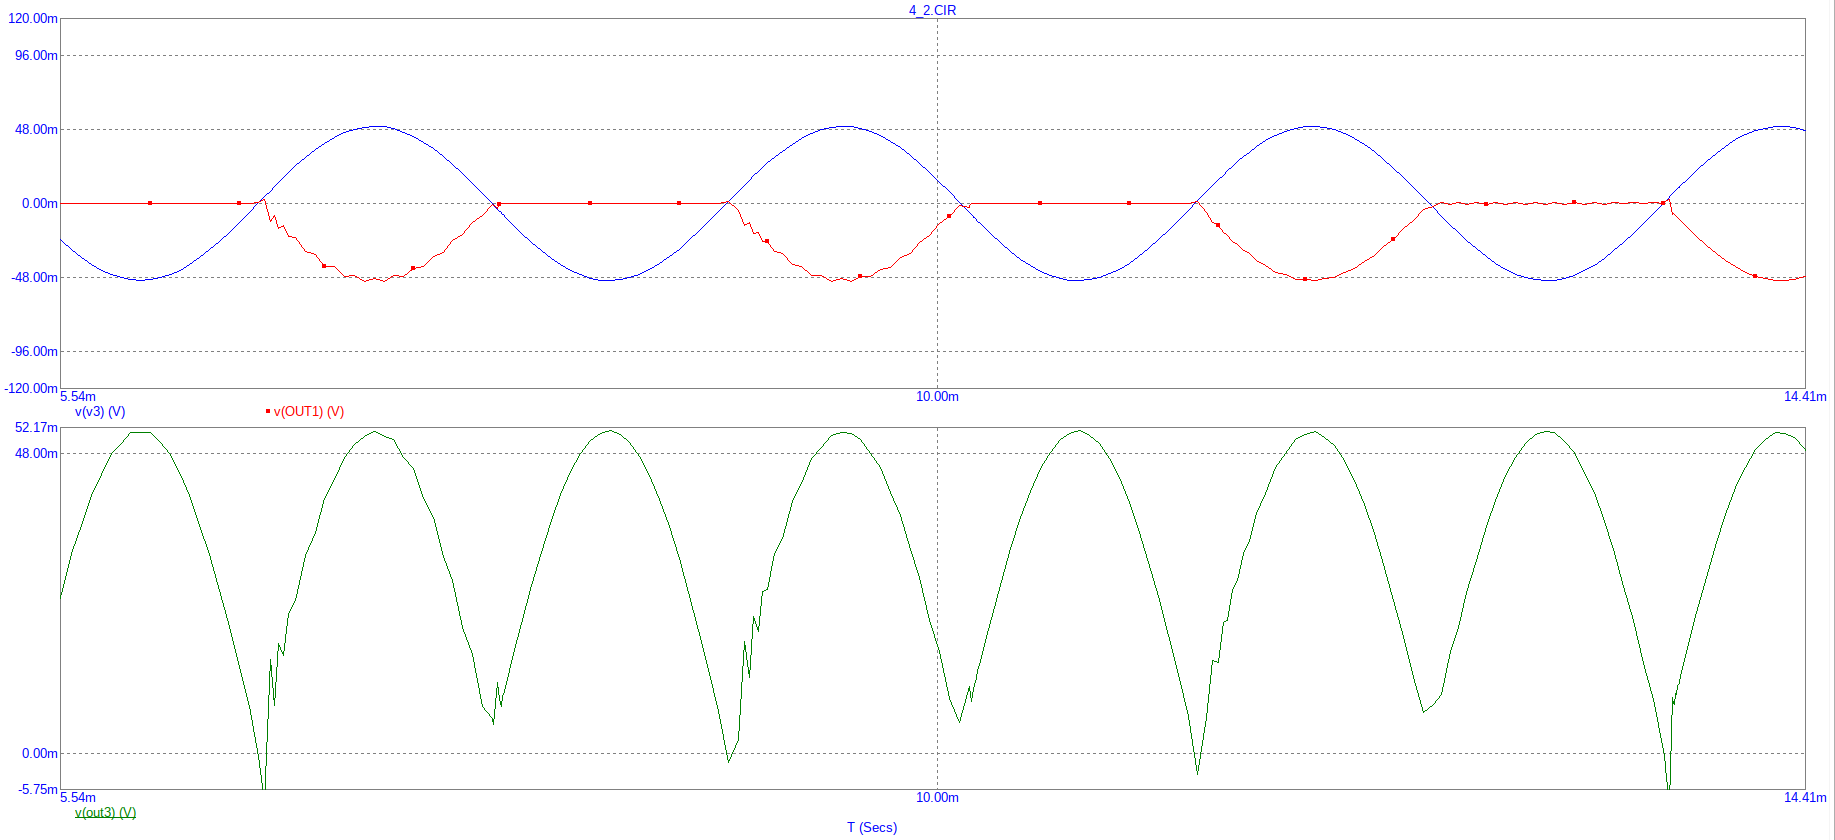
\includegraphics[width=0.7\textwidth]{microcap/2-transient-420hz-0.05v.png}
    \caption{Zapojení b) -- časová závislost napětí na výstupech obou OZ na vstupním napětí, nejnižší amplituda, při které uspokojivě usměrňuje, \(f=\qty{420}{\hertz}, U_M=\qty{50}{\milli\volt}\).}
    \label{fig:microcap/.png}
\end{figure}

\begin{figure}[h!]
    \centering
    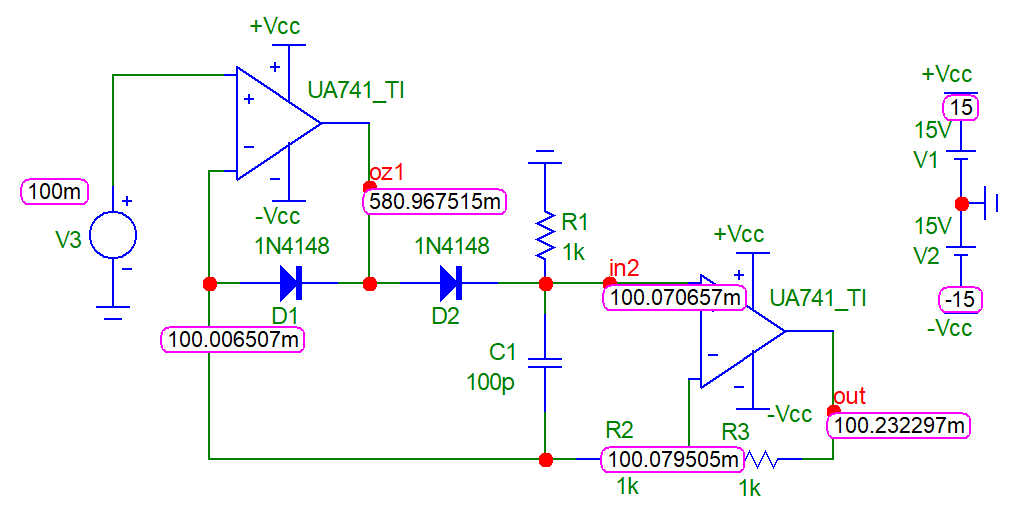
\includegraphics[width=0.8\textwidth]{microcap/3-dcbod.png}
    \caption{Zapojení c) -- stejnosměrný prac. bod při kladném napětí na vstupu, na výstupu kladné napětí.}
    \label{fig:microcap/.png}
\end{figure}

\begin{figure}[h!]
    \centering
    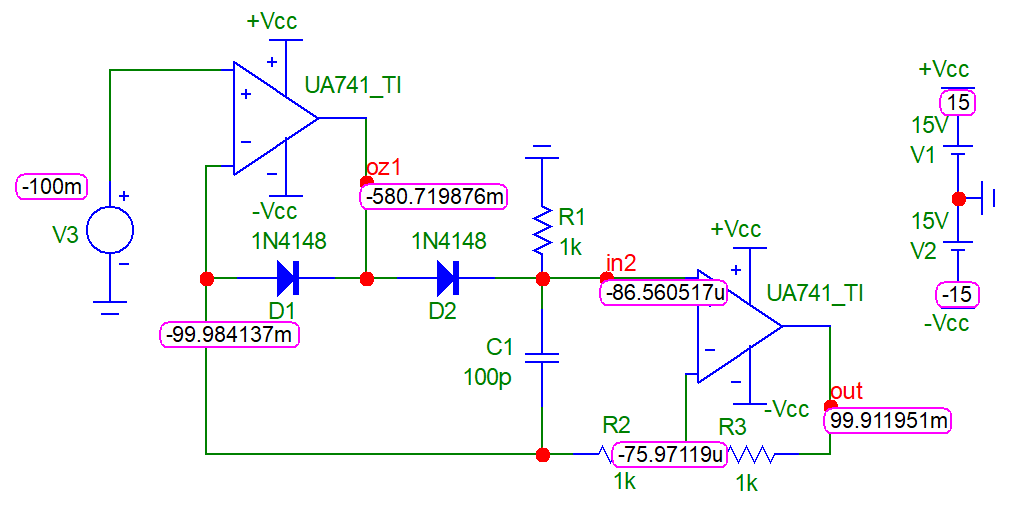
\includegraphics[width=0.8\textwidth]{microcap/3-dcbod2.png}
    \caption{Zapojení c) -- stejnosměrný prac. bod při záporném napětí na vstupu, na výstupu kladné napětí.}
    \label{fig:microcap/.png}
\end{figure}

\begin{figure}[h!]
    \centering
    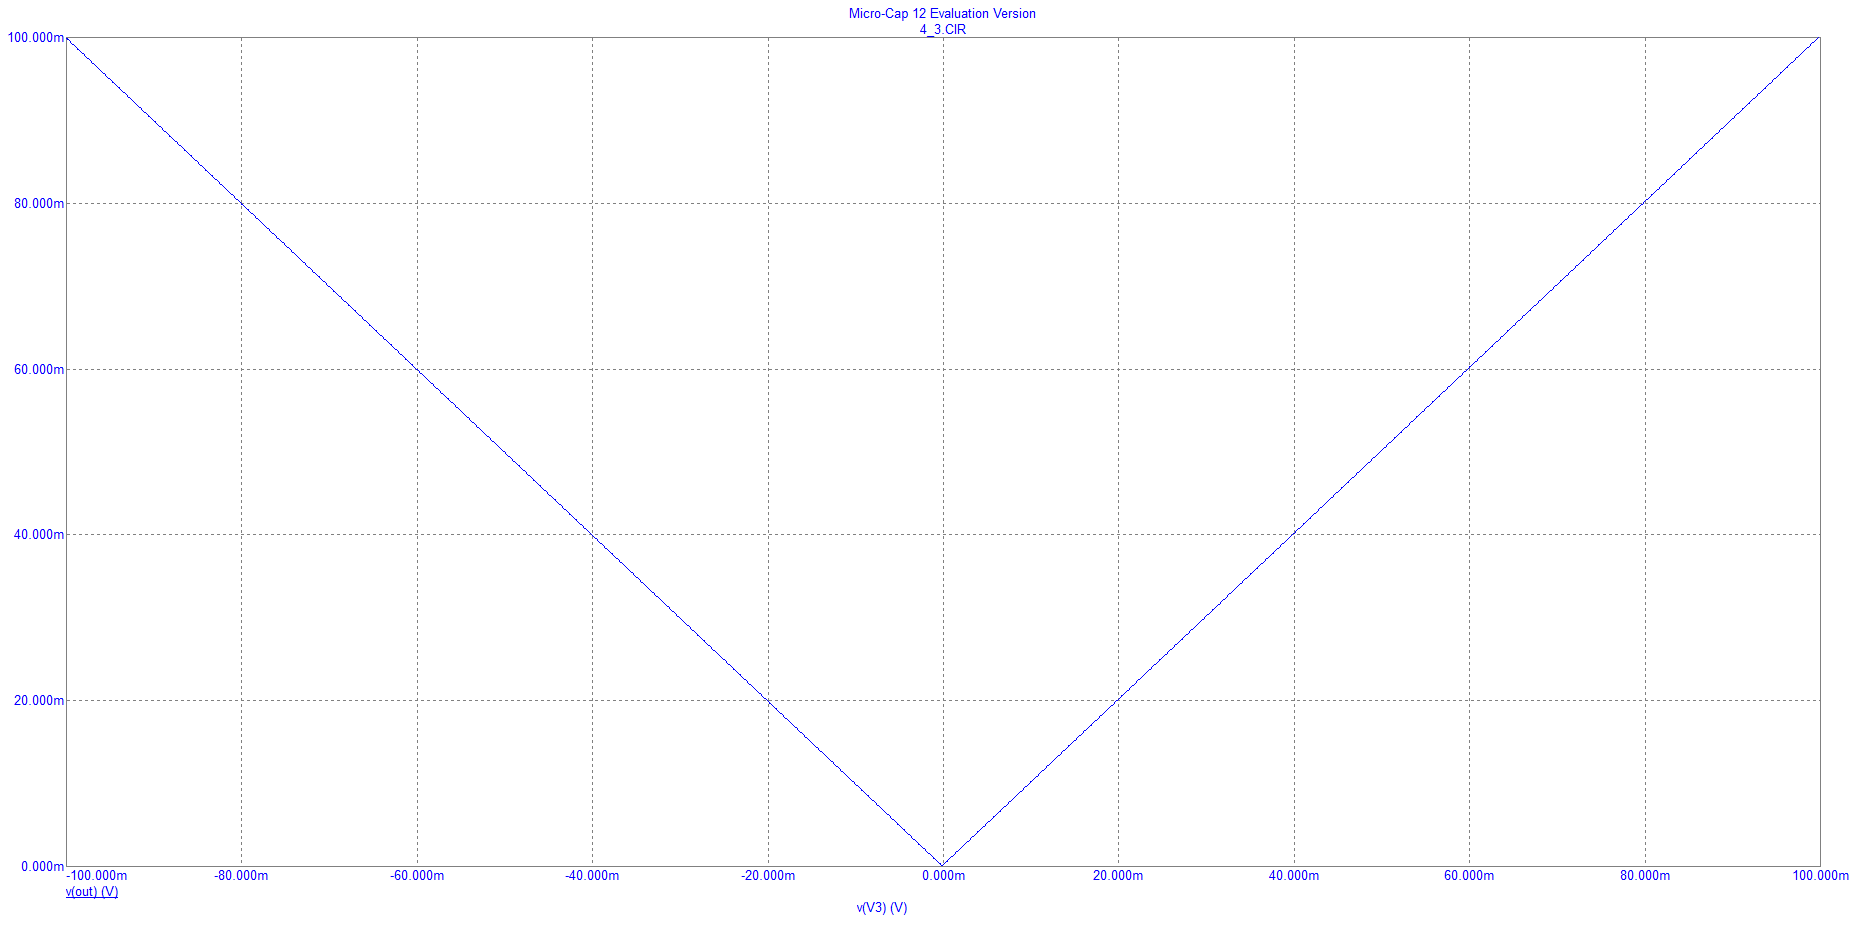
\includegraphics[width=0.8\textwidth]{microcap/3-dcprevodni.png}
    \caption{Zapojení c) -- stejnosměrná převodní charakteristika.}
    \label{fig:microcap/.png}
\end{figure}

\begin{figure}[h!]
    \centering
    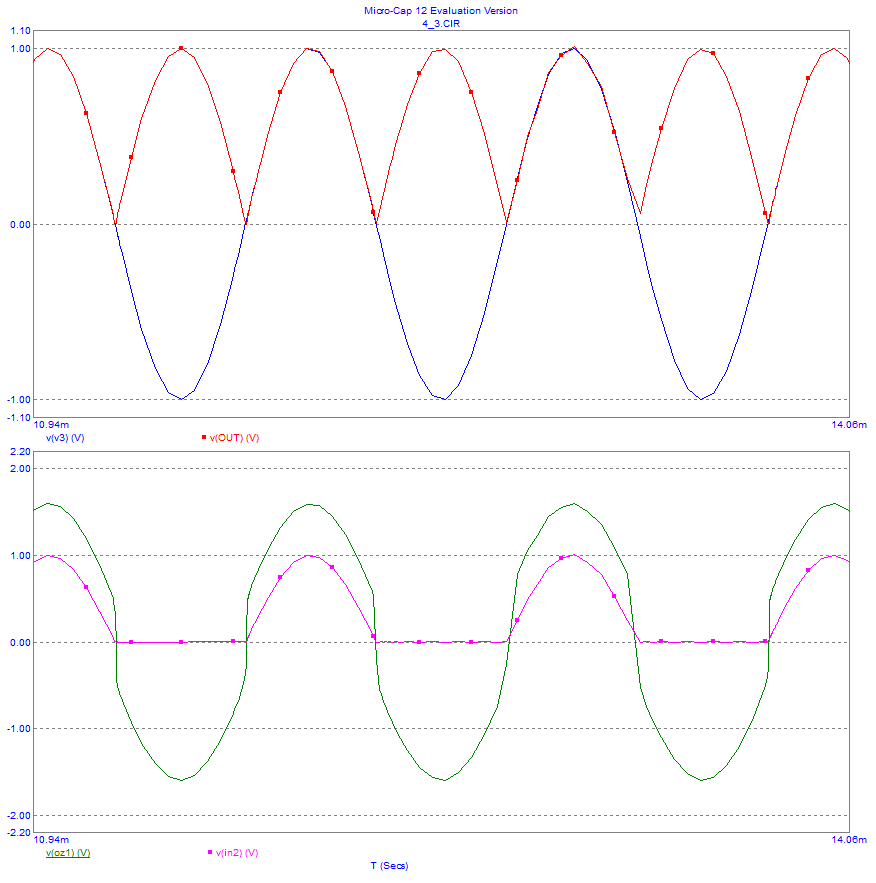
\includegraphics[width=0.66\textwidth]{microcap/3-transient-1khz-1v.png}
    \caption{Zapojení c) -- časová závislost napětí na výstupech obou OZ na vstupním napětí, jednocestné a dvoucestné usměrnění, \(f=\qty{1}{\kilo\hertz}, U_M=\qty{1}{\volt}\).}
    \label{fig:microcap/.png}
\end{figure}

\begin{figure}[h!]
    \centering
    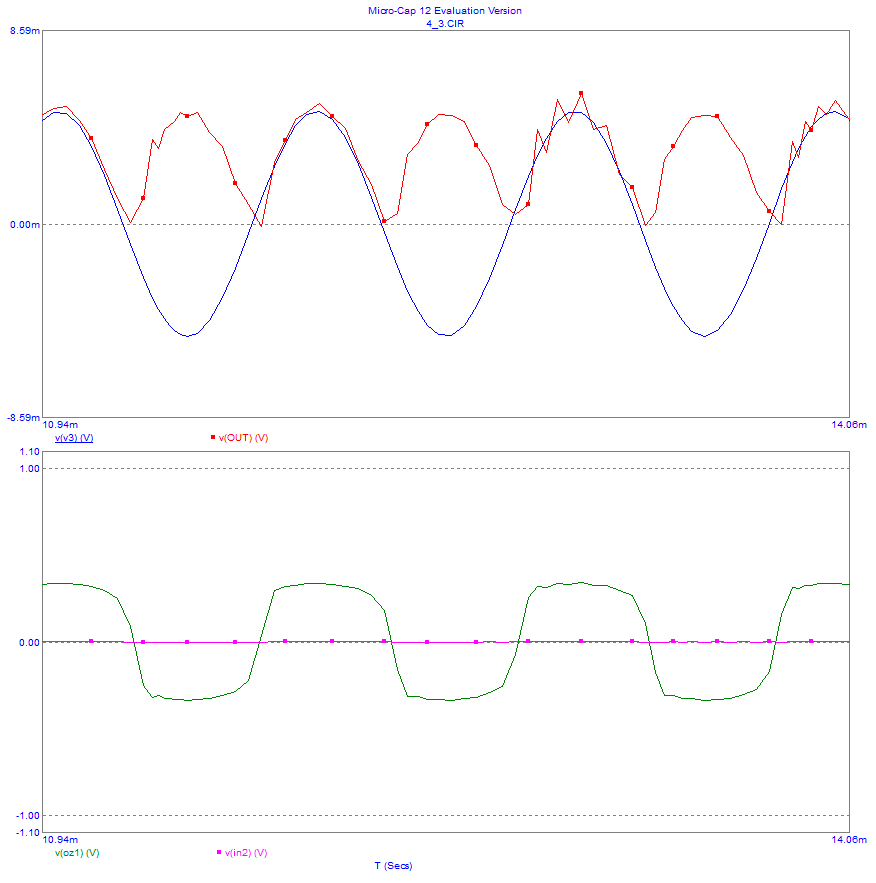
\includegraphics[width=0.66\textwidth]{microcap/3-transient-1khz-5mv.png}
    \caption{Zapojení c) -- časová závislost napětí na výstupech obou OZ na vstupním napětí, nejnižší amplituda, při které uspokojivě usměrňuje, \(f=\qty{1}{\kilo\hertz}, U_M=\qty{5}{\milli\volt}\).}
    \label{fig:microcap/.png}
\end{figure}

% \begin{figure}[h!]
%     \centering
%     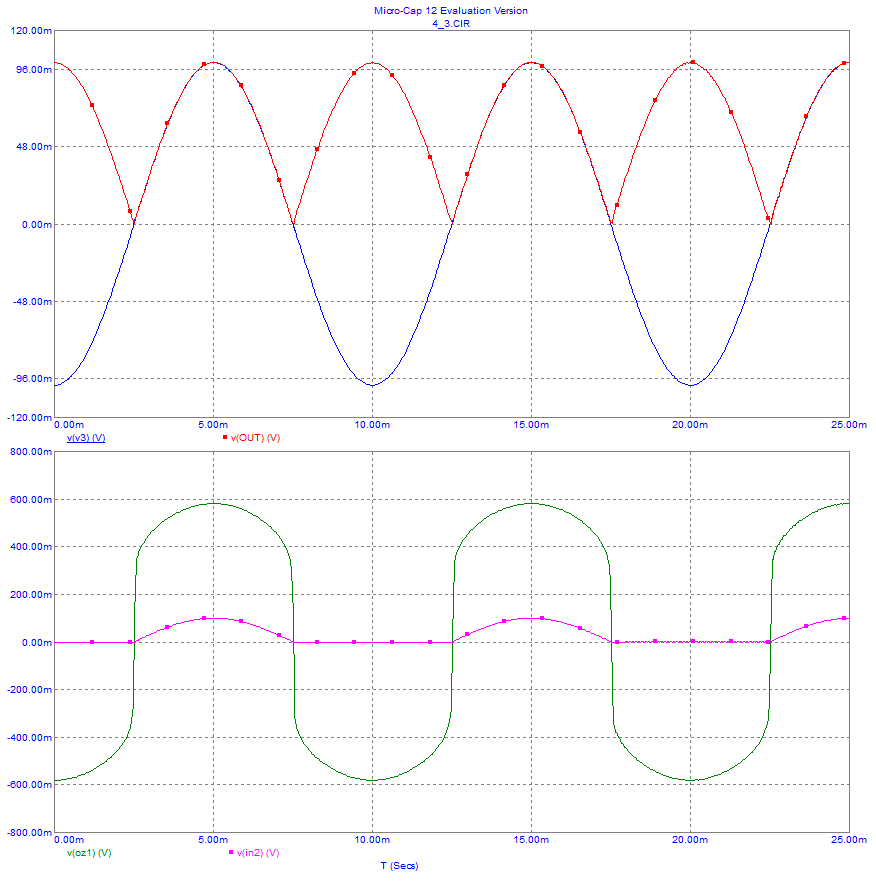
\includegraphics[width=0.8\textwidth]{microcap/3-transient-100hz-0.1v.png}
%     \caption{microcap/.png}
%     \label{fig:microcap/.png}
% \end{figure}

\begin{figure}[h!]
    \centering
    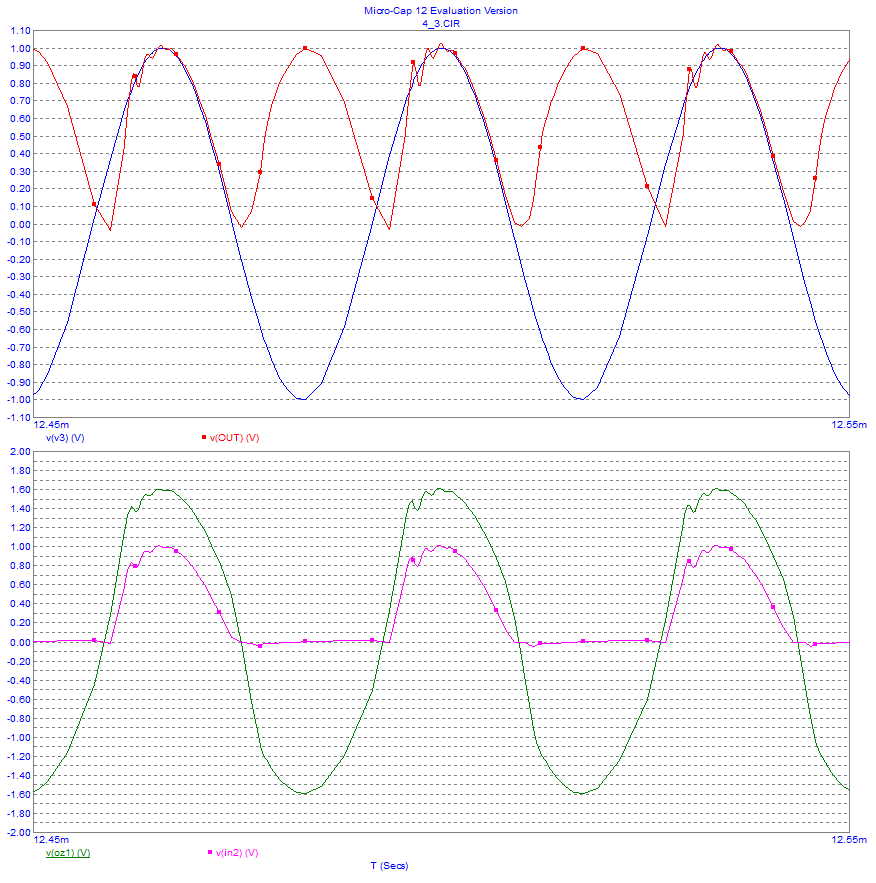
\includegraphics[width=0.8\textwidth]{microcap/3-transient-30khz-1v.png}
    \caption{Zapojení c) -- časová závislost napětí na výstupech obou OZ na vstupním napětí, nejvyšší frekvence, při které uspokojivě usměrňuje, \(f=\qty{30}{\kilo\hertz}, U_M=\qty{1}{\volt}\).}
    \label{fig:microcap/.png}
\end{figure}


%		

%	\clearpage

\section{Zpracování měřených hodnot}

\begin{figure*}[h!]
	\begin{tikzpicture}
		\centering
		\begin{axis}
			[
			xlabel={\( U\ [\unit{\volt}]\)},
			ylabel={\( I\ [\unit{\ampere}]\)},
			%axis y line*=left, % dve y osy
			width=1\textwidth,
			height = 0.5\textwidth,
			legend pos=south west,
%			xmin=0,
%			ymin=0,
%			xmax=100
%			ymax=100
			]

			\addplot[mark=x, mark options={solid}, thick, blue, only marks, mark size=3pt] table [skip first n=1, x=Unast, y=I, col sep=comma] {data/VA-bila.csv};
			\addlegendentry{Nastavené napětí}
			\addplot[mark=+, mark options={solid}, thick, red, only marks, mark size=3pt] table [skip first n=1, x=U, y=Inast, col sep=comma] {data/VA-bila.csv};
			\addlegendentry{Nastavený proud}
			
			% \addlegendentry{}
			
		\end{axis}   
	 
		 
	\end{tikzpicture}
	\caption{VA charakteristika při bílém světle.}
\end{figure*}


\begin{figure*}[h!]
	\begin{tikzpicture}
		\centering
		\begin{axis}
			[
			xlabel={\( U\ [\unit{\volt}]\)},
			ylabel={\( I\ [\unit{\ampere}]\)},
			%axis y line*=left, % dve y osy
			width=1\textwidth,
			height = 0.5\textwidth,
			legend pos=south west,
%			xmin=0,
%			ymin=0,
%			xmax=100
%			ymax=100
			]

			\addplot[mark=x, mark options={solid}, thick, blue, only marks, mark size=3pt] table [skip first n=1, x=Unast, y=I, col sep=comma] {data/VA-cervena.csv};
			\addlegendentry{Nastavené napětí}
			\addplot[mark=+, mark options={solid}, thick, red, only marks, mark size=3pt] table [skip first n=1, x=U, y=Inast, col sep=comma] {data/VA-cervena.csv};
			\addlegendentry{Nastavený proud}
			
			% \addlegendentry{}
			
		\end{axis}   
	 
		 
	\end{tikzpicture}
	\caption{VA charakteristika při červeném světle.}
\end{figure*}


\begin{figure*}[h!]
	\begin{tikzpicture}
		\centering
		\begin{axis}
			[
			xlabel={\( U\ [\unit{\volt}]\)},
			ylabel={\( I\ [\unit{\ampere}]\)},
			%axis y line*=left, % dve y osy
			width=1\textwidth,
			height = 0.5\textwidth,
			legend pos=south west,
%			xmin=0,
%			ymin=0,
%			xmax=100
%			ymax=100
			]

			\addplot[mark=x, mark options={solid}, thick, blue, only marks, mark size=3pt] table [skip first n=1, x=Unast, y=I, col sep=comma] {data/VA-zelena.csv};
			\addlegendentry{Nastavené napětí}
			\addplot[mark=+, mark options={solid}, thick, red, only marks, mark size=3pt] table [skip first n=1, x=U, y=Inast, col sep=comma] {data/VA-zelena.csv};
			\addlegendentry{Nastavený proud}
			
			% \addlegendentry{}
			
		\end{axis}   
	 
		 
	\end{tikzpicture}
	\caption{VA charakteristika při zeleném světle.}
\end{figure*}


\begin{figure*}[h!]
	\begin{tikzpicture}
		\centering
		\begin{axis}
			[
			xlabel={\( U\ [\unit{\volt}]\)},
			ylabel={\( I\ [\unit{\ampere}]\)},
			%axis y line*=left, % dve y osy
			width=1\textwidth,
			height = 0.5\textwidth,
			legend pos=south west,
%			xmin=0,
%			ymin=0,
%			xmax=100
%			ymax=100
			]

			\addplot[mark=x, mark options={solid}, thick, blue, only marks, mark size=3pt] table [skip first n=1, x=Unast, y=I, col sep=comma] {data/VA-modra.csv};
			\addlegendentry{Nastavené napětí}
			\addplot[mark=+, mark options={solid}, thick, red, only marks, mark size=3pt] table [skip first n=1, x=U, y=Inast, col sep=comma] {data/VA-modra.csv};
			\addlegendentry{Nastavený proud}
			
			% \addlegendentry{}
			
		\end{axis}   
	 
		 
	\end{tikzpicture}
	\caption{VA charakteristika při modrém světle.}
\end{figure*}


\begin{table}[]
	\centering
	\def\arraystretch{1.4}
	\begin{tabular}{|c|c|c|c|}
			\hline
			Veličina & \(U_{OC}\ [\unit{\volt}] \)  &  \(I_{SC}\ [\unit{\milli\ampere}]\) &  \(P_{max}\ [\unit{\milli\watt}]\)  \\ \hline \hline
			Bílá & 1,98 &  12,6 &  14,11 \\\hline
			Červená & 1,86 &  5,4 &  6,22 \\\hline
			Zelená & 1,86 &  4,8 &  5,15 \\\hline
			Modrá & 1,9 &  9,2 &  11,04 \\\hline
	\end{tabular}
	\caption{Naměřené hodnoty \(U_{OC} \) a \(I_{SC} \).}
	\label{tab:tabulka-hodnot}
\end{table}

	\clearpage
\section{Závěr}


\end{document}